\documentclass[12pt]{jarticle}
\usepackage[a4paper,text={155mm,230mm},centering]{geometry}
\usepackage{amssymb,amsmath,amsthm}
\usepackage{amsmath}
%\usepackage[dvips]{graphicx}
\usepackage{fancyhdr}
\pagestyle{fancy}
\lhead{ワイヤレス給電システムの最適化のための能率的な動作周波数スイープ}
\chead{}
\rhead{\thepage}
\lfoot{}
\cfoot{}
\usepackage{empheq}
\rfoot{森田光流}
\usepackage{fancybox}
\usepackage{listings,jlisting}
\usepackage{color}
\usepackage{ascmac, here, txfonts, txfonts}
\usepackage[dvipdfmx]{graphicx}
\usepackage{here}
\usepackage{multirow}

\begin{document}
	
%%%%%%%%%%%%%%%%%%%%%%%%%%%%%%%%%表紙
\thispagestyle{empty}

\vspace*{20mm}
\begin{center}
	{\Large 令和元年度 環境ロボティクス学科 卒業論文}
\end{center}
\vspace{10mm}
\begin{center}
	{\Huge ワイヤレス給電システムの最適化のための能率的な動作周波数スイープ}
\end{center}
\vspace{90mm}
\begin{center}
	{\Large 令和2年 (2020) 2月14日}
\end{center}
\begin{center}
	{\Large 森田 光流}
\end{center}
\begin{center}
	{\Large 指導教員:穂高一条教授}
\end{center}

\clearpage
%%%%%%%%%%%%%%%%%%%%%%%%目次

\tableofcontents

\clearpage
%%%%%%%%%%%%%%%%%%%%%%%本文

\section{緒言}
\subsection{背景}
\subsubsection{ワイヤレス給電の概要}
ワイヤレス給電とは,コネクタや金属接点の接触を用いず無線で電力を供給,伝搬することが可能な給電方法である.非接触充電,非接触電力送電,無線給電などとも呼ばれている.従来の電気製品の給電方法の金属接点やコネクタを使用したものは,水がかかると水による感電やショートを起こす,配線による転倒などの安全面に関して問題点がある.しかしワイヤレス給電は金属接点が非接触なので前述に述べた安全面の問題点の解決するだけではなく,人が立ち入れない危険な場所にある機器や装置の遠隔操作ができるなどという利点が期待されており,現在盛んに研究されている.
\subsubsection{ワイヤレス給電の特徴}
ワイヤレス給電が無線で電力を供給するためには,送電側と受電側の2つのコイルを用いるため物理的な金属接点やコネクタが存在せず,また非金属のものであれば,コイル間に存在していても送電側と受電側の電力に影響を及ぼさない.また,送電コイルを表面に露出させる必要がないため,水による感電やショートする心配がないので,水場での使用が可能である.なお,ワイヤレス給電の給電方式には送電側と受電側との間発生する誘導磁束を利用した電磁誘導方式や,キャパシタを送電電極と受電電極として電力を送電する電解結合方式などがある\cite{rohm2}\cite{ito}が,本研究ではその中の電磁共鳴方式で行う.
\subsubsection{ワイヤレス給電の将来性}
現在,ワイヤレス給電の特徴を生かして様々な場所に導入しようと 研究が行われている.前述に述べた通り金属接点が非接触なので,ワイヤレス給電化することにより物理的な金属接点が少なくなるので電源コードは最小限で済み余分な空間を作ることにより直接配線などの問題解決並びに自動化・効率化に大きく貢献している\cite{syourai}\cite{matuda}.
\\ また,地球温暖化の影響によりCO{\tiny 2}の削減のため電気自動車開発並びに普及が望まれている.現在,電気自動車に使用されている接触式充電方式は雨天時にプラグを扱うと感電する可能性がある.それをワイヤレス給電に置き換えると自宅の駐車場に駐車するだけで充電が可能になり電の可能性が払拭される,充電の際に運転者が降車する必要がなくなり運転者の負担が大きく軽減されることが期待される.\cite{hakugin}
\clearpage
\subsection{研究目的}
ワイヤレス給電の電力供給の効率の改善には,
\\1.最適な周波数調整
\\2.結合操作
\\3.マルチループコイルとLC回路を用いた適応マッチング
\\などがある\cite{morita}.本研究においては1.に注目し,そのために最適動作周波数の探索をすることとした.1.を最適動作周波数を探索するには,受電電力と送電電力を使った電力効率を求める必要がある.しかし,電力効率が高いだけでは最適動作周波数が適切であるとはいえない.受電側と送電側の元々の電力が小さい場合も電力効率が高いということが考えられる.それではワイヤレス給電が最適に動作しているとは考えられない.したがって,最適動作周波数は高効率かつ大電力が出力される周波数と定義される.
\\ また最適動作周波数を探索するためには多くの周波数を測定しなければいけないので測定時間をなるべく短くしたい.しかし,ワイヤレス給電に周波数を送った後,安定な電力が出力されるまで時間がかかる.したがって本研究は能率的な周波数スイープ設計し,
ワイヤレス給電システムの最適動作周波数を能率的な周波数スイープによる測定,考察を目的にした.
\clearpage
\section{本論文の構成}
\subsection*{緒言}
	本研究の背景および,研究目的をこの章で述べる.
\subsection*{本研究での基礎理論と原理} ワイヤレス給電についての原理,または本研究において扱うワイヤレス給電測定による基礎理論についてを述べる.
\subsection*{実験内容}
	本研究で使用した実験道具の条件,プログラム・システムについての説明,計測前のシミュレーション結果についてをこの章で述べる.
\subsection*{実験結果}
	本研究の実験結果について述べる.
\subsection*{結言}
	実験結果に対しての考察, 今後の展望について述べる.
\clearpage
\section{本研究での基礎理論と原理}
\subsection{ワイヤレス給電の原理}
\begin{figure}[h]
	\centering
	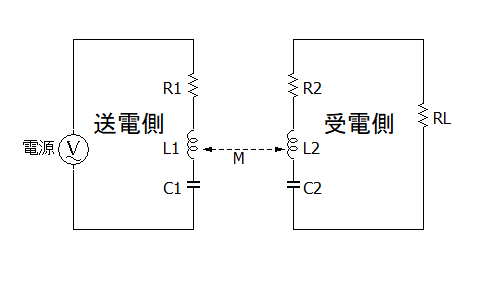
\includegraphics[]{wpt_2020128.png}
	\caption{ワイヤレス給電回路図}
	\label{fig:wpt_kairo}
\end{figure}
本研究で扱うワイヤレス給電の回路は図\ref{fig:wpt_kairo}で示される.図\ref{fig:wpt_kairo}に示すように,ワイヤレス給電は送電側と受電側が電気的につながっていないことが分かる.送電側の交流電源の電流が時間的に変化することにより受電側の磁束が変化しファラデーの電磁誘導の法則より受電側に誘導起電力が生じ誘導電流を伝えるという原理である.また,図\ref{fig:wpt_kairo}の回路素子は以下の通りである.
\begin{quote}
	\begin{itemize}
		\item L1:送電側のコイルの自己インダクタンス.
		\item L2:受電側のコイルの自己インダクタンス.
		\item M:送電側と受電側のコイルの相互インダクタンス.
		\item R1:送電側コイルの内部抵抗
		\item R2:受電側コイルの内部抵抗
		\item C1:送電側のコンデンサの電気容量
		\item C2:受電側のコンデンサの電気容量
		\item RL:受電側の負荷抵抗
		\item 電源:送電側回路の交流電源
	\end{itemize}
\end{quote}
\clearpage
\subsection{共振周波数}
 周波数と電力の関係として,共振周波数について説明する.共振周波数は回路が共振するときの周波数である.本研究において図\ref{fig:RLC}のRLC直列回路を使用する.この場合はRLC直列回路の共振周波数になる.
\begin{figure}[H]
	\centering
	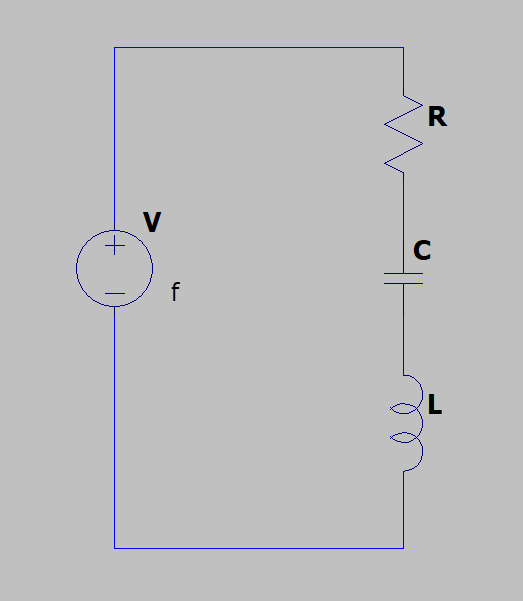
\includegraphics[scale=0.5]{RLC.png}
	\caption{RLC直列回路}
	\label{fig:RLC}
\end{figure}
共振周波数を求めるためにはまずインピーダンスを求める必要がある.図\ref{fig:RLC}の時インピーダンスは,
\begin{eqnarray}
\label{eq:Z}
\dot{Z}=R+j(X_L-X_C) \nonumber\\
=R+j(\omega L-\frac{1}{\omega C})
\end{eqnarray}
となる.このとき$\omega$は角周波数であり,
\begin{equation}
\label{eq:omega}
\omega=2 \pi f
\end{equation}
となる.RLC直列回路が直列共振する条件は,\ref{eq:Z}の$X_L-X_Cが0になるときなので$
\begin{eqnarray}
\omega L-\frac{1}{\omega C}=0 \nonumber \\
\label{eq:zyouken}
\omega L=\frac{1}{\omega C}
\end{eqnarray}
\begin{equation}
\dot{Z}=R
\label{eq:R}
\end{equation}
となる.またその時の周波数を$f_0$とし,式(\ref{eq:omega})式(\ref{eq:zyouken})から,
\begin{equation}
2 \pi f_0L=\frac{1}{2 \pi f_0C}
\label{eq:f_0}
\end{equation}
式(\ref{eq:f_0})から$f_0を解くと$
\begin{eqnarray}
f_0=\frac{1}{2 \pi\sqrt{LC}}
\label{eq:kyousin}
\end{eqnarray}
となる.
\\ 式(\ref{eq:R}),図\ref{fig:RLCkyosin}からRLC直列回路が共振周波数近づくほどインピーダンスが小さくなり遠くなるほど大きくなる.インピーダンスが小さいと電流が大きくなる.したがって周波数が共振周波数のとき最も電力が大きいことが分かる.
\begin{figure}[H]
	\centering
	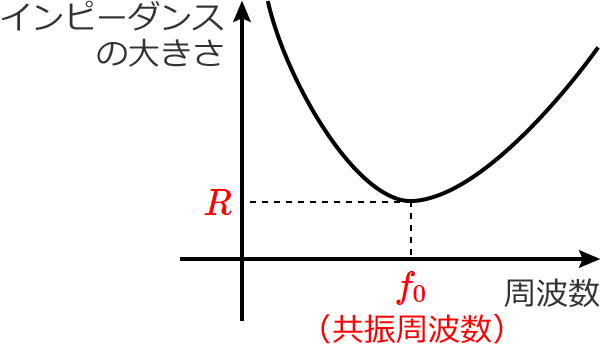
\includegraphics[scale=0.5]{RLCkyousin.png}
	\caption{周波数とインダクタンスの関係}
	\label{fig:RLCkyosin}
\end{figure}
\subsection{平均電力・効率}
ワイヤレス給電の最適動作周波数を探索するためには平均電力と効率を求める必要があるが,平均電力を求めるにはワイヤレス給電の定常解を求める必要がある.
\subsubsection{定常解の導出}
状態方程式は,一般的に
\begin{equation}
\label{eq:zyoutai}
\dot{x}=Ax+Bu
\end{equation}
と表せられる.(ワイヤレス給電の状態方程式の求め方は後述の付録参照)
\\ この式(\ref{eq:zyoutai})を解くと,
\begin{equation}
e^{-At}\dot{x}(t)-e^{-At}Ax(t)=e^{-At}Bu(t)
\end{equation}
記号の都合により,$tを\tau$にして求めると,
\begin{eqnarray}
\frac{d}{d\tau}(e^{-A\tau}x(\tau))=e^{-A\tau}Bu(\tau)\\
\left[e^{-A\tau}x(\tau)\right]^t_0=\int_{0}^{t}e^{-A\tau}Bu(\tau)d\tau\\
e^{-At}x(t)-x(0)=\int_{0}^{t}e^{-A\tau}Bu(\tau)d\tau\nonumber\\
e^{-At}x(t)=x(0)+\int_{0}^{t}e^{-A\tau}Bu(\tau)d\tau
\end{eqnarray}
$両辺にe^{At}をかけると,$
\begin{equation}
\label{eq:siki}
x(t)=e^{-At}x(0)+e^{-At}\int_{0}^{t}e^{-A\tau}Bu(\tau)d\tau
\end{equation}
となり,式(\ref{eq:siki})は状態方程式の一般解である.平均電力と効率は状態方程式の周期的な解に基づくため,式を周期的な関数にしなければならない.したがって$x(t)が周期Tをもつ関数とすると,$
\begin{equation}
\label{eq:T}
x(t+T)=x(t)
\end{equation}
となり,式(\ref{eq:T})に式(\ref{eq:siki})を代入して整理すると,
\begin{equation}
\label{eq:muzu}
x(0)=(I-e^{AT})^{-1}e^{A(T-t)}\int_{0}^{T}e^{-A\tau}Bu(t+\tau)d\tau-\int_{0}^{t}e^{-A\tau}Bu(\tau)d\tau
\end{equation}
で求まる(但し,$det(1-e^{AT}\neq0)$の時だけ).式(\ref{eq:muzu})を式(\ref{eq:siki})に代入し,周期解$x_{ss}(t)$を求めると,
\begin{eqnarray}
x_{ss}(t)=e^{At}(I-e^{AT})^{-1}e^{A(T-t)}&\int_{0}^{T}e^{-A\tau}Bu(t+\tau)d\tau&-\int_{0}^{t}e^{-A\tau}Bu(\tau)d\tau+\int_{0}^{t}e^{-A\tau}Bu(\tau)d\tau\nonumber\\
x_{ss}(t)=(I-e^{AT})^{-1}e^{At}&\int_{0}^{T}e^{-A\tau}Bu(t+\tau)d\tau&
\label{eq:Tteizyou}
\end{eqnarray}
よって,周期$T$定常解は式\ref{eq:Tteizyou}で求められる.
\subsubsection{短形波入力の場合の定常解}
短形波入力の定義は,
\begin{eqnarray}
u(t ) &=& 
\begin{cases}
u_0 \quad &(0\leqq t <Td)  \\
0 \quad &(Td\leqq t <T) 
\end{cases}
\nonumber
\\
\label{eq:tannkei}
かつ\quad u(t)&=&u(t+T)
\end{eqnarray}
であらわされる.$T$は1周期であり$d$はデューティー比である.そこから式(\ref{eq:Tteizyou})に式(\ref{eq:tannkei})を代入し範囲ごとに場合分けで積分し,$x_{sst}(t)$を求める.
\\ \qquad i. $0\leqq t<Tdの場合$
\begin{gather}
\int_{0}^{T}e^{-Ap}Bu{t+p}dp=\int_{0}^{Td-t}e^{-Ap}Bu(t+p)dp+\int_{Td-t}^{T-t}e^{-Ap}Bu(t+p)dp+\int_{T-t}^{T}e^{-Ap}Bu{t+p}dp\nonumber \\
=\int_{0}^{Td-t}e^{-Ap}Bu_0dp+\int_{T-t}^{T}e^{-Ap}Bu_0dp \nonumber \\ 
=-A^{-1}e^{-AT}(e^{A(t+T(1-d))}-e^{-At}-e^{AT}+I)Bu_0
\label{eq:0<td}
\end{gather}
\qquad ii. $Td \leqq t <Tdの場合$
\begin{gather}
\int_{0}^{T}e^{-Ap}Bu(t+p)dp=\int_{0}^{T-t}e^{-Ap}Bu(t+p)dp+\int_{T-t}^{t+dt-t}e^{-Ap}Bu(t+p)dp+\int_{T+dt-t}^{T}e^{-Ap}
Bu(t+p)dp \nonumber\\
=\int_{T-t}^{T+dt-t}e^{-Ap}Bu_0dp \nonumber\\
=-A^{-1}e^{-AT}(e^{A(t-td)}-e^{At})Bu_0
\label{eq:td<T}
\end{gather}
となる.よって,式(\ref{eq:0<td})と式(\ref{eq:td<T})から$x_{sst}(t)$は,
\begin{eqnarray}
x_{sst}(t)=
\begin{cases}
	-(I-e^{AT})^{-1}A^{-1}(e^{A(t+T(1-d))}-e^{At}-e^{AT}+I)Bu_o &\quad (0\leqq t <Td)\\
	-(I-e^AT)^)(-1))(e^{A(t-Td)}-e^{At})Bu_0 & \quad(Td\leqq t <T)
	\label{eq:tannkei}
\end{cases} 
\end{eqnarray}
となる.
\subsubsection{平均電力と電力効率の導出}
ある時刻においての電力を瞬時電力というが,平均電力は時間範囲内でその瞬時電力を時刻ごと加算して平均したものである.ここでは計算での平均電力と電力効率を求める方法を述べる \\ある時刻においての瞬間電力$p_t$,電圧$v$,電流$i$とおくと
\begin{equation}
p_t=vi
\end{equation}
と表すことができる.瞬間電力が周期$T$をもつ場合,平均電力は0から$T$まで積分し,そして$T$で割ることにより求められる.よって,
\begin{equation}
P=\frac{1}{T}\int_{0}^{T}p_tdt
\end{equation}
となる.また,送電側と受電側の瞬時電力は次のように表される.
\begin{eqnarray}
\label{eq:ui_1}
p_{t1}=ui_1\\
\label{eq:R_Li_2^2}
p_{t2}=R_Li_2^2
\end{eqnarray}
一次側と二次側の平均電力は式(\ref{eq:ui_1})と式(\ref{eq:R_Li_2^2})より
\begin{eqnarray}
\label{eq:P1}
P_1=\frac{1}{T}\int_{0}^{T}u(t)i_1(t)dt\\
\label{eq:P2}
P_2=\frac{1}{T}\int_{0}^{T}R_Li_2^2dt
\end{eqnarray}
と導くことができる.\\
 このように正弦波のような連続の関数を持つ周期関数はそのまま式(\ref{eq:P1})と式(\ref{eq:P2})に代入することが可能だが,短形波の平均電力は連続ではないので,注意して求める必要がある.したがって短形波の平均電力を求めるには,式(\ref{eq:zyoutai})の状態方程式と式(\ref{eq:tannkei})の短形波の定常解を使って解くと,
 \begin{eqnarray}
 P_1=\frac{1}{T}\int_{0}^{Td}ui_{1ss1}(t)dt\\
 P_2=\frac{1}{T}R_L(\int_{0}^{Td}i_{2ss1}^2dt+\int_{Td}^{T}i_{2ss2}^2dt)
 \end{eqnarray}
 となる.また$i_{1ss1},i_{2ss1}は0 \leqq t < Tdのときのi_1,i_2でi_{2ss2}はTd \leqq t <Tのときのi_2である.$また,電力効率は$求めたP_1,P_2より$
 \begin{equation}
 \eta=\frac{P_2}{P_1}\\
 \label{eq:kouritu}
 \end{equation}
 と求まる.これにより,送電側と受電側の平均電力と効率を求められる.
 \clearpage
 \subsection{実験における平均電力の求め方}
 前の小節にも述べた通り,最適動作周波数を求めるには送電側と受電側の平均電力と効率を求めなければならない.平均電力を求めるためには積分を使わなければいけない.そこで,以下の方法が挙げられる.
 \begin{figure}[h]
 	\centering
 	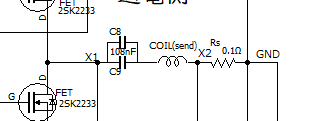
\includegraphics[]{191127shunt.png}
 	\caption{送電側回路測定部分}
 	\label{fig:shunt}
 \end{figure}
\\ 図(\ref{fig:shunt})に示されているものは,送電側の回路図上にシャント抵抗$R_s$を加えたものである.コイルに通る電流を$i$,シャント抵抗の抵抗は$R_s=0.1\Omega$なので,シャント抵抗間の電圧は,
\begin{equation}
v_s=0.1i
\end{equation}
となる.\\
 電力を求めるにはシャント抵抗の電圧とコイル間電圧$V_L$を乗算器でかけることにより求めることができる.実験で使用した乗算器は乗算した値が1/10倍出力される特性を持つから,オペアンプでシャント抵抗の電圧を100倍にすることが求められる.$v_s$を100倍された値は,
\begin{equation}
0.1i \times 100=10i
\end{equation}
となる.
 \begin{figure}[h]
	\centering
	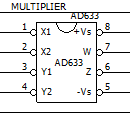
\includegraphics[]{191127zouhuku.png}
	\caption{乗算器回路図}
	\label{fig:zouhuku}
\end{figure}
 \\ \\図(fig:zouhuku)の乗算器回路において,計算方法としては以下のとおりである.
\begin{eqnarray}
W=\frac{(X1-X2)(Y1-Y2)}{10}+Z
\end{eqnarray}
$コイル間電圧V_Lの電位のX1とX2を乗算器のX1とX2,オペアンプを通した後の電圧を乗算器のY1,回路のGNDをY2とすると,$図(fig:shunt)上での電力の以下のようになる.なお,図(\ref{fig:zouhuku})のZはGNDにつないでいる.
\begin{eqnarray}
W=\frac{(X1-X2)(Y1-Y2)}{10}+Z \nonumber \\
=\frac{(X1-X2)(10V_s-0)}{10}+0 \nonumber \\
=\frac{V_L10i}{10i}=V_Li
\end{eqnarray}
となり実験中で電力を求めることができる.
\begin{figure}[H]
	\centering
	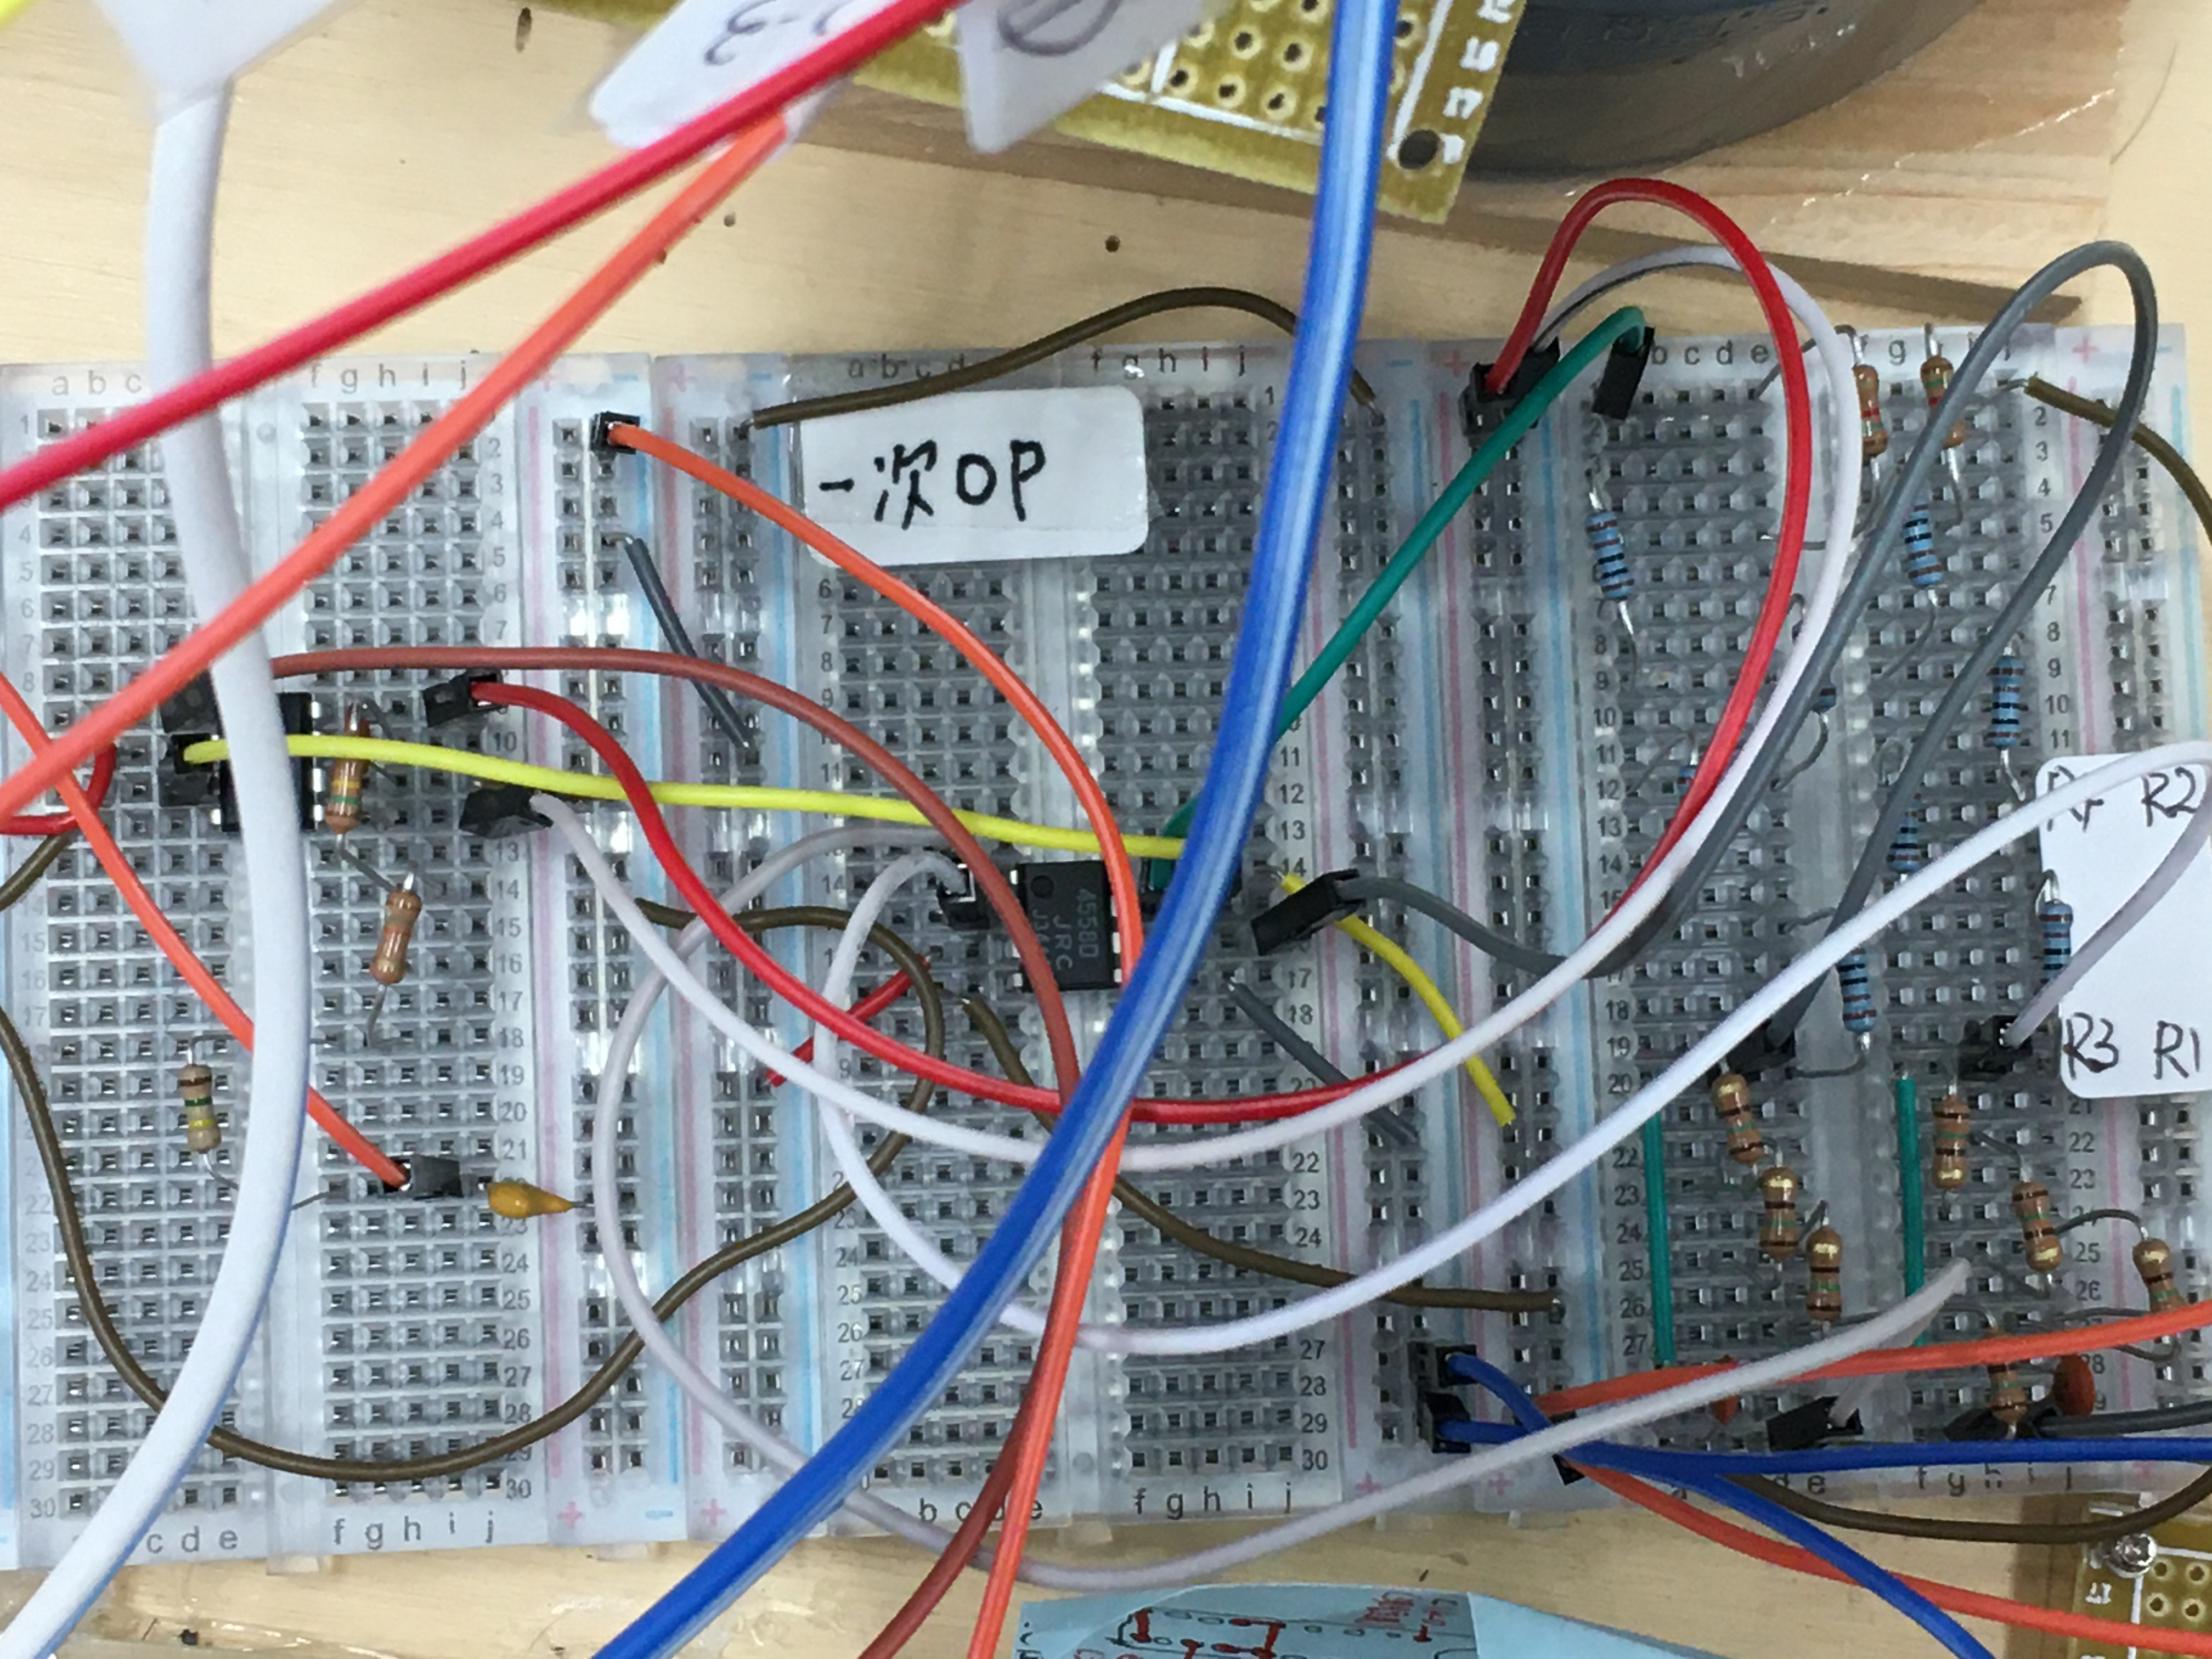
\includegraphics[scale=0.1,angle=180]{op_multi.JPG}
	\caption{オペアンプー乗算器回路}
	\label{fig:op_multi}
\end{figure}
 \clearpage
\section{実験内容}
\subsection{周波数スイープの概要}
 実験による最適動作周波数を探索する方法としては周波数スイープが挙げられる.周波数スイープとは一定の時間や速度において周波数を変化させ出力させる方法である.なお本研究における周波数スイープは以下のようなやり方でする.(図\ref{fig:freq_sweep})
 \begin{figure}[H]
	\centering
	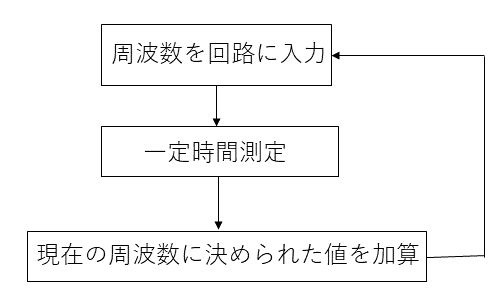
\includegraphics[]{freqency_sweep.png}
	\caption{周波数スイープ方法図}
	\label{fig:freq_sweep}
\end{figure}
\begin{enumerate}
	\item 一番最初の周波数を回路に送る.なお一番最初の周波数,一番最後の周波数,1つの周波数における測定時間,次の周波数で加算する周波数(以後加算周波数)の量をあらかじめ決めておく必要がある.
	\item 決めた時間で測定する.0.1秒ずつデータが出力される.
	\item 一定時間に達したら,加算周波数を加算し一番最後の周波数に達するまで繰り返す.
\end{enumerate}
\clearpage
\subsection{プログラムによる周波数スイープ自動化}
先行研究では,ワイヤレス給電の周波数スイープをArduinoだけで実行した.しかしArduinoだけでは周波数や時間を変更する時,わざわざコンパイルしなければならず面倒であった.そこで本研究では周波数スイープの周波数を送る,ワイヤレス給電の電力を受け取る作業をpythonで自動化させるようにした.\\
	一連の操作は以下の箇条書きと図\ref{fig:zidouka}のとおりである.
 \begin{figure}[H]
	\centering
	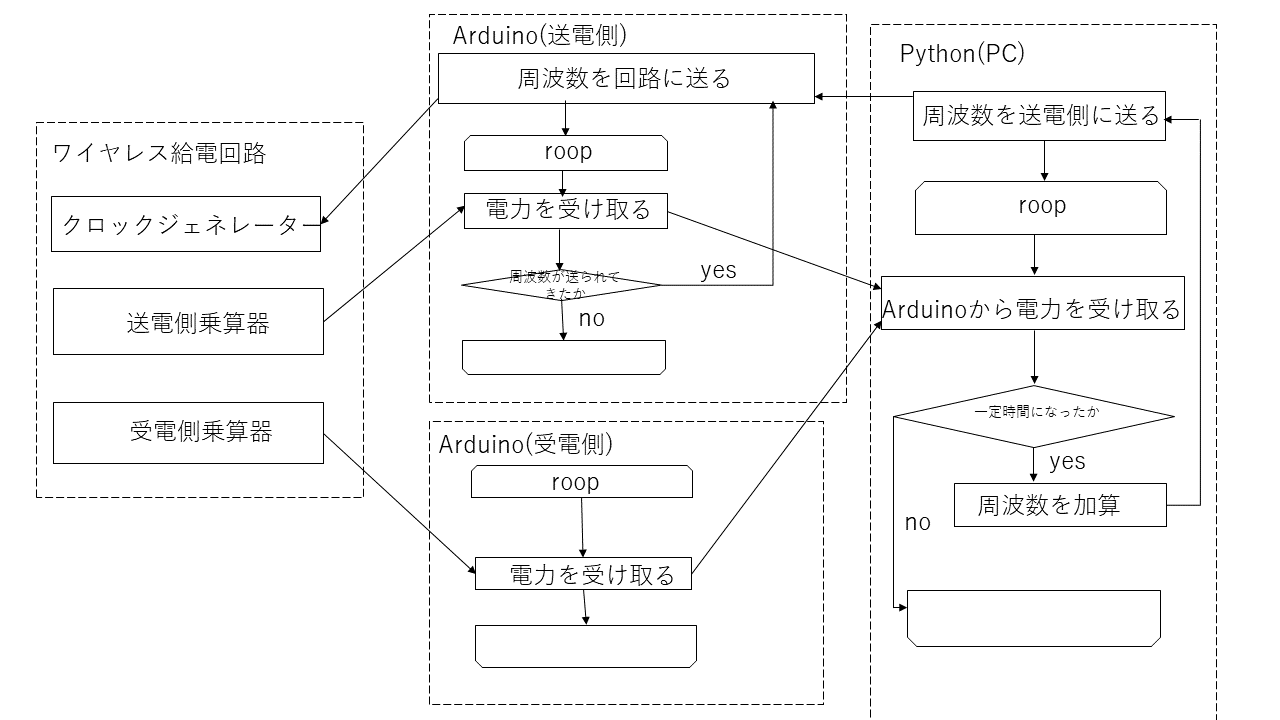
\includegraphics[scale=0.4]{huro.png}
	\caption{周波数スイープ自動化のフローチャート}
	\label{fig:zidouka}
\end{figure}
	\begin{enumerate}
		\item pythonによって送られてきた周波数の値を送電側のArduinoで,ワイヤレス給電回路の中にある短形波を出力することができるクロックジェネレータへ指定した周波数を送る.
		\item 乗算器によって出力された電力を送電側・受電側のArduinoにデューティー比で送る.また送られたデューティー比を電力に直す.
		\item 電力をpythonへ送りデータを保存する.また自分が指定した時間が経ったら周波数を変えて,送りなおす.
		\item 1~3までの一連の操作を最後の周波数になるまで送り続ける.
	\end{enumerate}
	以上のような流れですべての周波数の時の電力の測定をする.また,最初の周波数,最後の周波数,周波数をなんHzずつ見るための加算する周波数,一つの周波数の電力を測定する時間をGUIで入力できるようにした.次の図(\ref{fig:gui})は本実験において使用したGUIである.また作成したpythonとarduinoのプログラムは本論文の付録に書かれている.
 \begin{figure}[H]
	\centering
	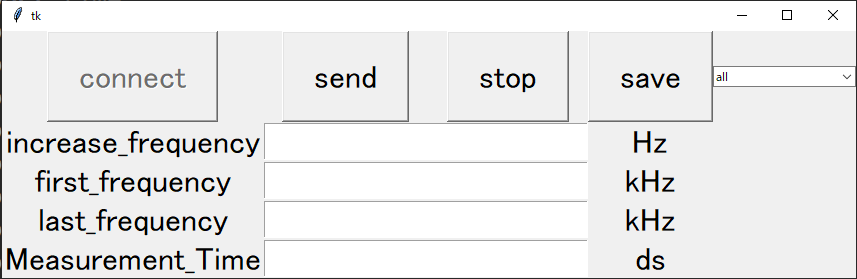
\includegraphics[scale=0.5]{gui.png}
	\caption{電力測定するためのGUI}
	\label{fig:gui}
\end{figure}
\clearpage
\subsection{最適動作判定}
ワイヤレス給電の最適動作周波数であるには前章にも述べたが高電力かつ高効率であることが重要である.したがって次の計算式を導入した.なお,定数はそれぞれ周波数スイープによって測定と受電側の電力$P_2,式(\ref{eq:kouritu})によって導き出された効率\eta$である.
\begin{eqnarray}
(最適動作判定)=P_2\eta
\end{eqnarray}
この値が高い数値であればあるほど最適動作周波数だといえる.
\subsection{能率的な周波数スイープ}
\subsubsection*{時間・加算周波数決定}
先行研究では,一つの周波数を送って測定するまでの時間を10秒で測定した.しかし,今研究においては多くの周波数を測りたいがためあまり時間をかけたくないから10秒では多すぎると考える.逆に測定時間を短くしすぎると出力される電力が周期的になるまで時間がかかるので周期的になる前に出力される.また低周波ずつ上げると確かに正確に測ることが可能だが同じく時間がかかる.逆に大雑把に周波数を取りすぎると最適周波数が分からなくなる.したがって周波数スイープが能率的になる周波数の測定時間と,加算周波数の量を事前に決めておく必要がある.事前に決めた数値は表\ref{tab:hyo1}である.
\begin{table}[h]
	\centering
	\caption{測定時間・加算周波数決定値}
	\label{tab:hyo1}
	\begin{tabular}{|l|r|}\hline
		測定時間  & 1.5s \\ \hline
		加算周波数 & 10kHz\\ \hline
	\end{tabular}
\end{table}
\clearpage
\subsection{実験条件}
 \begin{figure}[H]
	\centering
	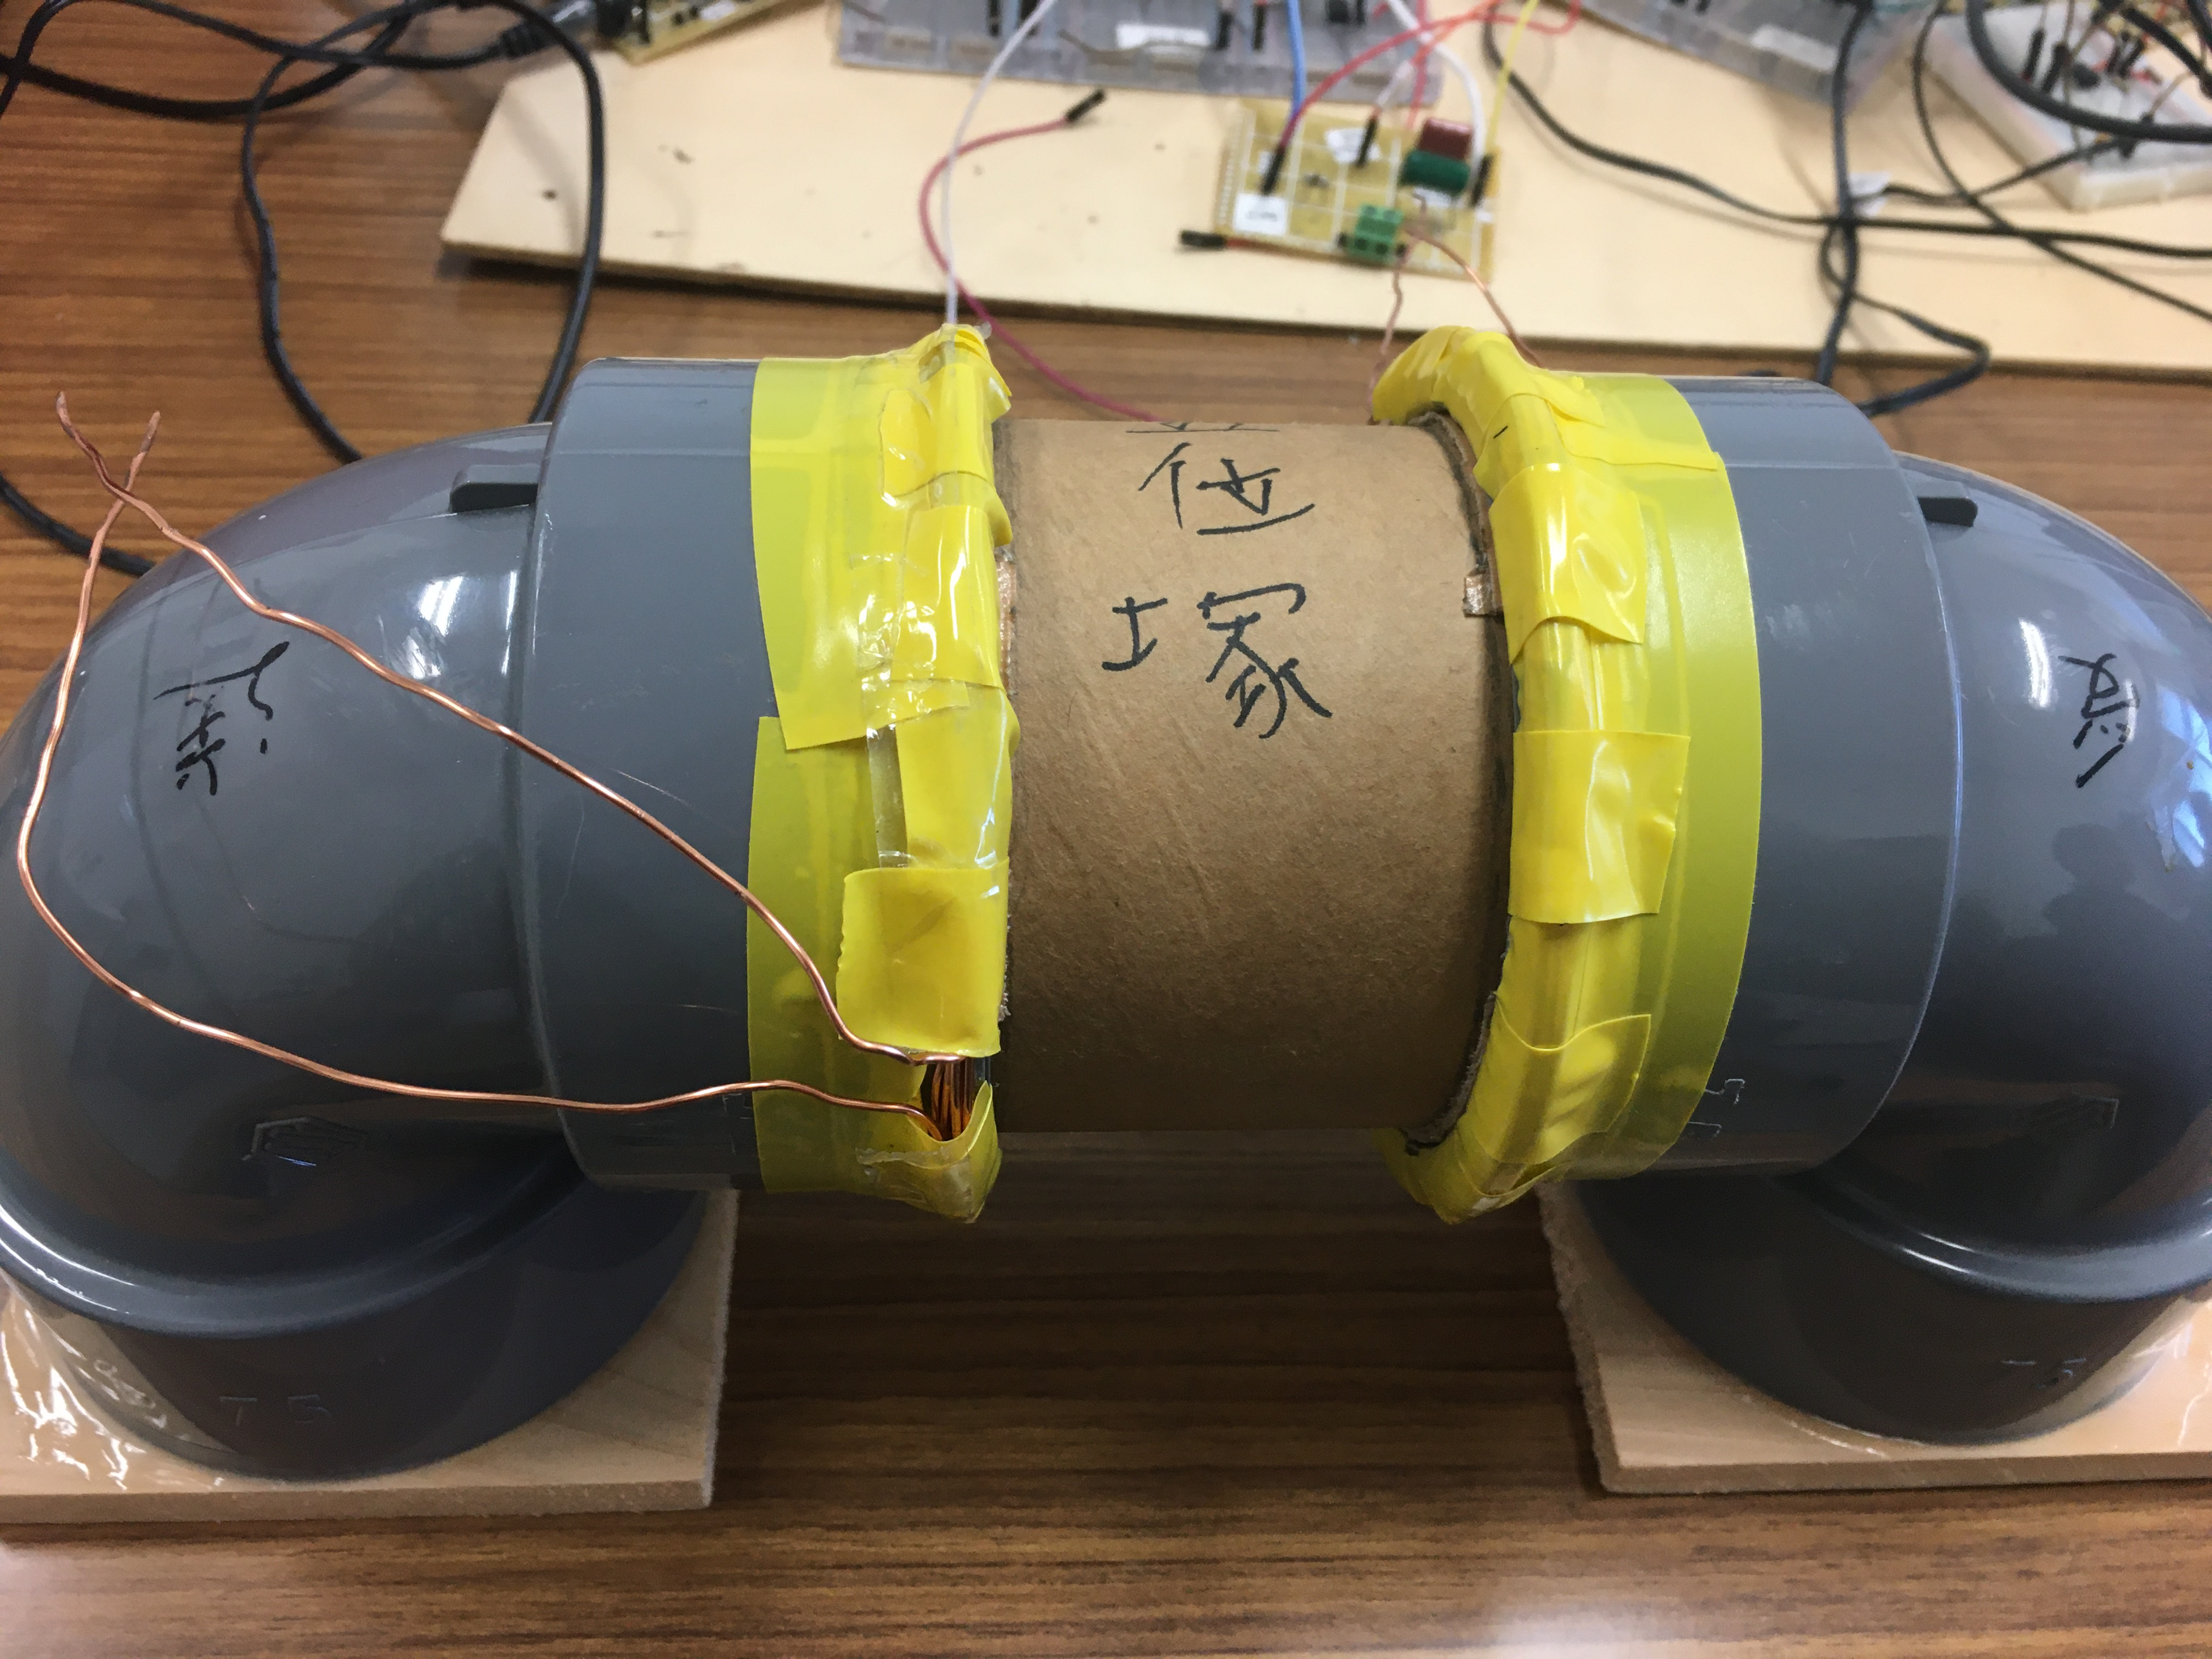
\includegraphics[scale=0.1]{koiru.JPG}
	\caption{実験コイル}
	\label{fig:koiru}
\end{figure}
本研究においてコイルは図\ref{fig:koiru}のものを使った.なおコイルは前々度の卒業研究(参考文献\cite{goizuka})で使われたものである.また,以下の表\ref{tab:koiru}において実験コイルの本体・インダクタンスのパラメータ,使用素子のパラメータの実験条件を示す.(参考文献:\cite{goizuka})また今回使用したクロックジェネレーター(図\ref{fig:clk})はおよそ4kHzより下の周波数は出力されないという性能も考慮して測定範囲は5kHzから100kHzとする.
また実験回路の共振周波数は式(\ref{eq:kyousin}),表\ref{tab:indact},表\ref{tab:sosi}より,送受電同じく,
\begin{equation}
f_0=\frac{1}{2\pi\sqrt{23.6\mu \times 108n}} 
\\=99.7kHz
\label{eq:99.6k}
\end{equation}

 \begin{figure}[H]
	\centering
	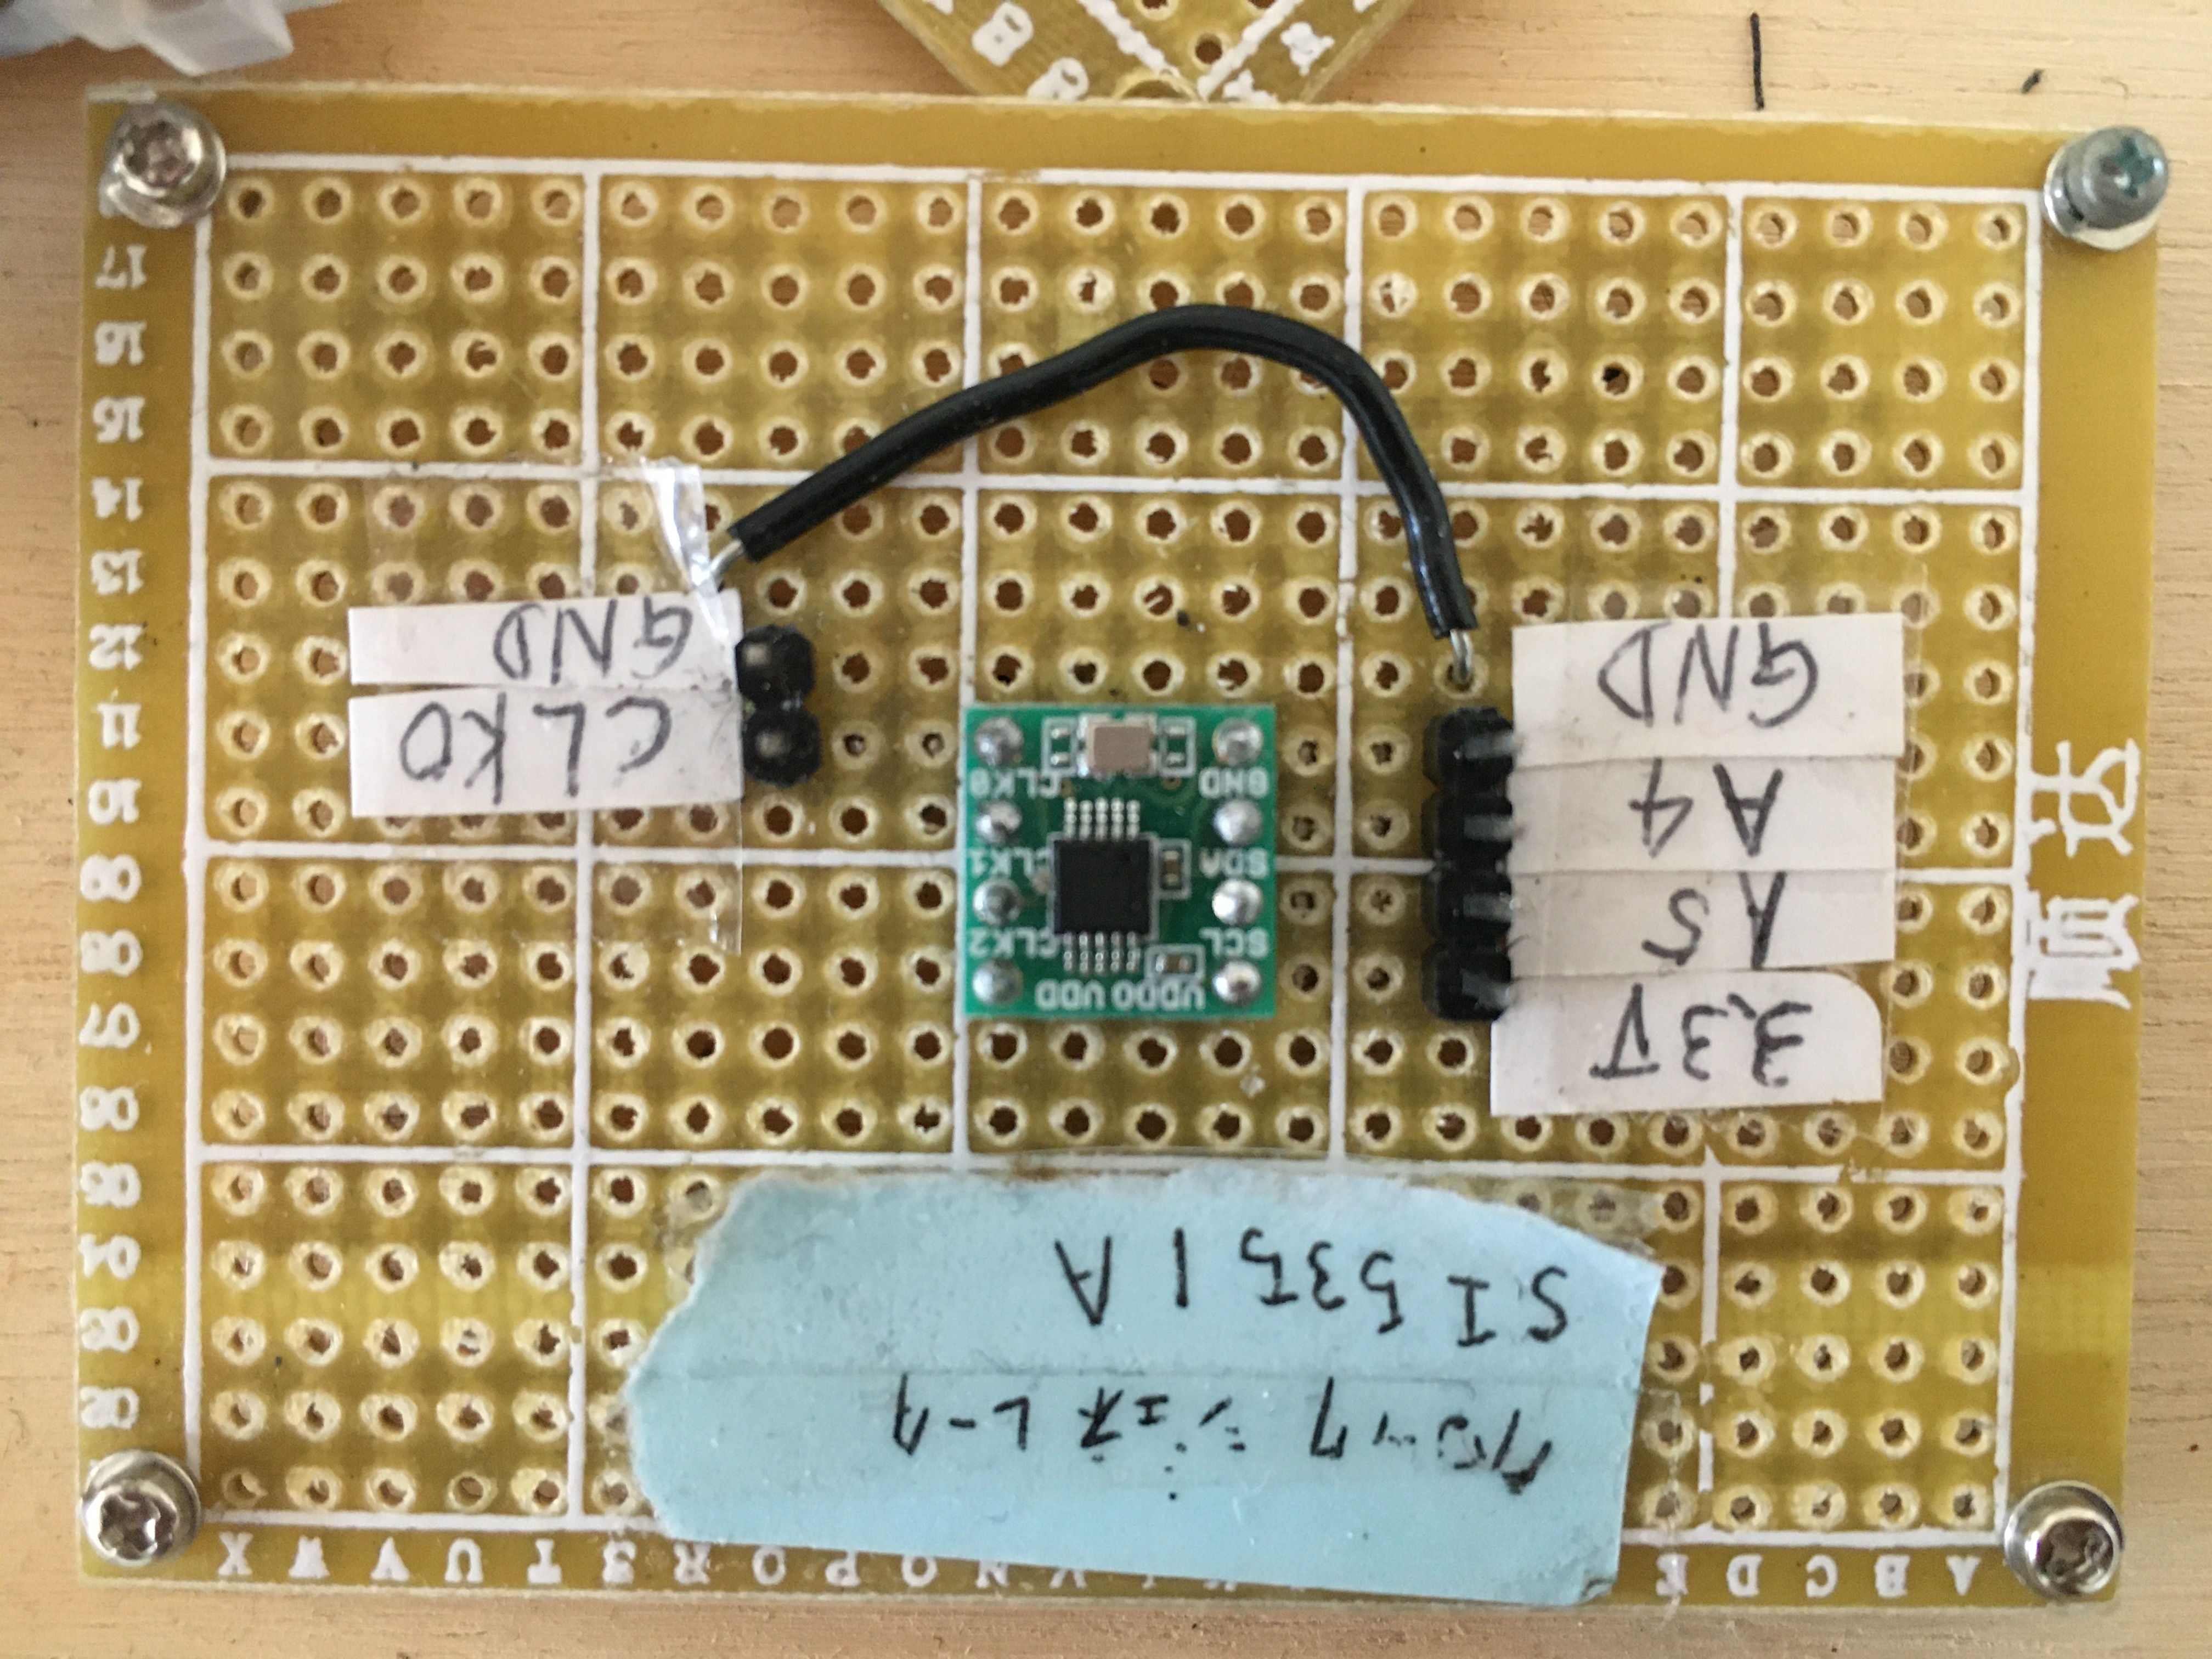
\includegraphics[scale=0.1,angle=180]{IMG_0737.JPG}
	\caption{クロックジェネレーター}
	\label{fig:clk}
\end{figure}
\begin{table}[h]
	\caption{実験コイル}
	\centering
	\label{tab:koiru}
	\begin{tabular}{|l|l|l|}
		\hline
		\multicolumn{2}{|l|}{パラメータ}          & 値{[}単位{]}                 \\ \hline
		\multirow{2}{*}{コイル半径}  & 送電側        & 0.05{[}m{]}               \\ \cline{2-3} 
		& 受電側        & 0.05{[}m{]}               \\ \hline
		\multirow{2}{*}{導線直径}   & 送電側        & 0.001{[}m{]}              \\ \cline{2-3} 
		& 受電側        & 0.001{[}m{]}              \\ \hline
		\multirow{2}{*}{送電側巻き数} & 同心         & 3{[}巻{]}                  \\ \cline{2-3} 
		& 垂直         & 3{[}巻{]}                  \\ \hline
		\multirow{2}{*}{受電側巻き数} & 同心         & 3{[}巻{]}                  \\ \cline{2-3} 
		& 垂直         & 3{[}巻{]}                  \\ \hline
		\multirow{2}{*}{抵抗}     & 送電側$(R_1)$ & 0.08($\Omega$) \\ \cline{2-3} 
		& 受電側$(R_2)$ & 0.08($\Omega$) \\ \hline
		\multicolumn{2}{|l|}{コイル間距離}      & 0.05{[}$m${]}                   \\ \hline
	\end{tabular}
\end{table}
\begin{table}[h]
	\centering
	\caption{コイルのインダクタンス}
	\label{tab:indact}
	\begin{tabular}{|l|l|l|}
		\hline
		\multicolumn{2}{|l|}{パラメータ}             & 値{[}単位{]}       \\ \hline
		\multirow{2}{*}{自己インダクタンス} & 送電側($L_1$) & 23.6{[}$\mu${]} \\ \cline{2-3} 
		& 受電側($L_2$) & 23.6{[}$\mu${]} \\ \hline
		相互インダクタンス                  & $M$        & 1.98{[}$\mu${]} \\ \hline
	\end{tabular}
\end{table}
\begin{table}[h]
	\centering
	\caption{使用素子}
	\label{tab:sosi}
	\begin{tabular}{|l|l|l|}
		\hline
		\multicolumn{2}{|l|}{パラメータ}       & 値{[}単位{]}                       \\ \hline
		電源電圧                   & $u$      & 10.0{[}$V${]}                   \\ \hline
		デューティ比                 & $d$      & 0.5                             \\ \hline
		\multirow{2}{*}{コンデンサ} & 送電側$C_1$ & 108{[}$nF${]}                   \\ \cline{2-3} 
		& 受電側$C_2$ & 108{[}$nF${]}                   \\ \hline
		負荷抵抗                   & $R_L$    & 20.0{[}\textbackslash{}Omega{]} \\ \hline
	\end{tabular}
\end{table}
\clearpage
\subsection{シミュレーション}
実験をする前に事前にシミュレートしてみた.図\ref{fig:simulatew}から図\ref{fig:simulatesaiteki}はそれぞれ電力出力,効率,最適動作判定の結果である..図\ref{fig:simulatesaiteki}からもわかる通りに,共振周波数は式(\ref{eq:99.6k})の近くの時,最適動作判定が最大だということが分かる.
 \begin{figure}[H]
	\centering
	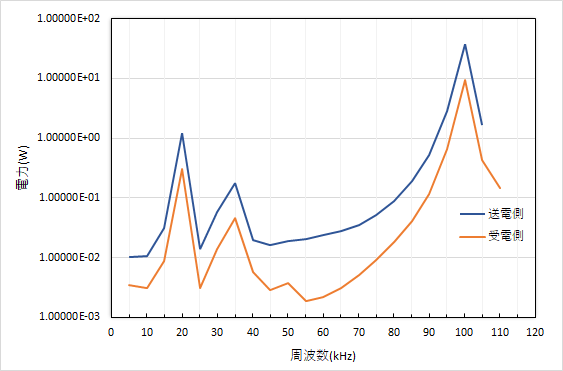
\includegraphics[scale=1]{シミュレーション電力.png}
	\caption{シミュレーション出力電力}
	\label{fig:simulatew}
\end{figure}
 \begin{figure}[H]
	\centering
	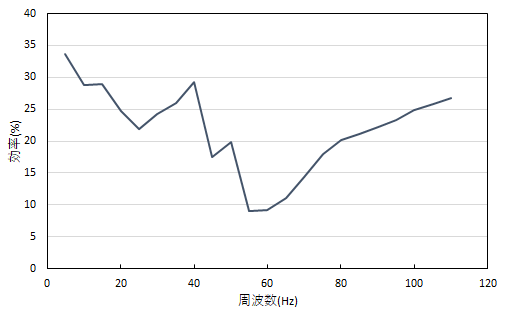
\includegraphics[scale=1]{kouritusimu.png}
	\caption{シミュレーションでの効率}
	\label{fig:simulatekou}
\end{figure}
 \begin{figure}[H]
	\centering
	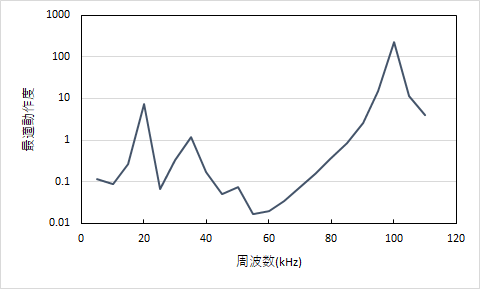
\includegraphics[scale=1]{saitekidousasimu.png}
	\caption{シミュレーションでの最適動作判定}
	\label{fig:simulatesaiteki}
\end{figure}
\clearpage
\section{実験結果}
\subsection{能率化してない周作数スイープ}
能率的な周波数スイープの比較材料として,能率化していない周波数スイープの場合も測定した.それぞれ図\ref{fig:not_nourituw},図 \ref{fig:not_nouritu_kou},図\ref{fig:not_nouritu_dousa}測定に用いた数値を表\ref{tab:not_nouritu}にある.
\begin{table}[H]
	\centering
	\label{tab:not_nouritu}
	\caption{能率化していない周波数スイープ測定時間と加算周波数}
	\begin{tabular}{|l|l|}
		\hline
		測定時間  & 10s \\ \hline
		加算周波数 & 1k  \\ \hline
	\end{tabular}
\end{table}
 \begin{figure}[H]
	\centering
	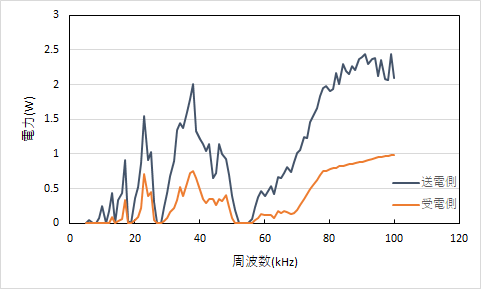
\includegraphics[]{not_nouritu_w.png}
	\caption{周波数と出力電力との関係}
	\label{fig:not_nourituw}
\end{figure}
\begin{figure}[H]
	\centering
	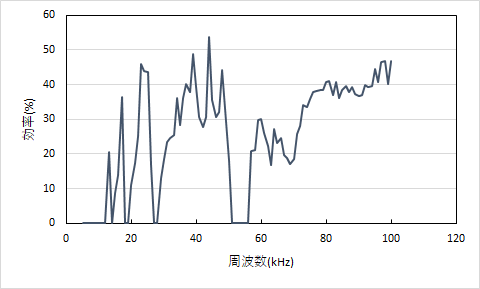
\includegraphics[]{notkouritu.png}
	\caption{周波数と効率の関係}
	\label{fig:not_nouritu_kou}
\end{figure}
\begin{figure}[H]
	\centering
	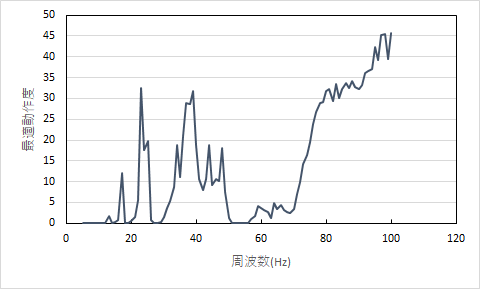
\includegraphics[]{not_nouritu_dousa.png}
	\caption{最適動作判定}
	\label{fig:not_nouritu_dousa}
\end{figure}
シミュレーションの結果と比べて送電側・受電側双方の電力が小さい値で出力された.
\subsection{能率的な周波数スイープ}
測定結果を以下のグラフに示す.
\begin{figure}[H]
\centering
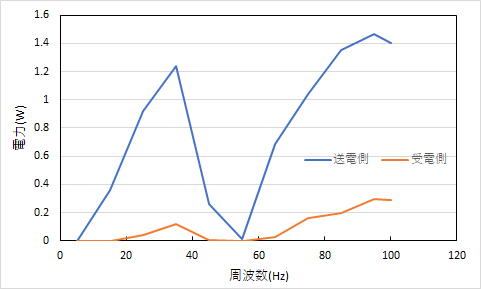
\includegraphics[]{nouritu_w.png}
\caption{周波数と出力電力との関係}
\label{fig:nourituw}
\end{figure}
\begin{figure}[H]
	\centering
	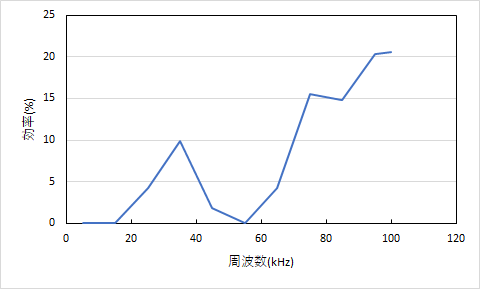
\includegraphics[]{nouritu_kou.png}
	\caption{周波数と効率の関係}
	\label{fig:nouritu_kou}
\end{figure}
\begin{figure}[H]
	\centering
	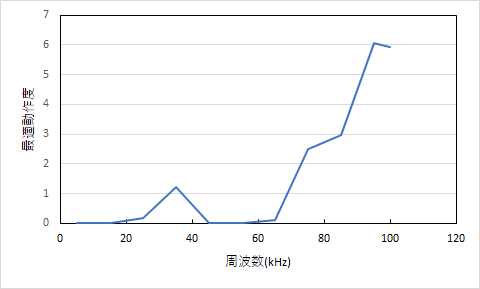
\includegraphics[]{nouritu_dousa.png}
	\caption{最適動作判定}
	\label{fig:nouritu_dousa}
\end{figure}
\clearpage
\section{結言}
\subsection{考察}

\clearpage
\subsection{今後の展望}
\clearpage
\section{謝辞}
 本研究の進行や本論文等の執筆にあたり,ご指導いただいた穂高一条教授に感謝の意を示すとともに深く御礼申し上げます.
また本研究を進めるにあたり多大な助言・アドバイスをしてくださった自動制御研究室の先輩である白銀聡一郎さん,大畑貴弘さん,橋本菜生さん,松浦健斗さん,並びに共に研究した同期のメンバーも感謝の意を示すとともに深く御礼申し上げます.最後になりましたが,お世話になりました宮崎大学工学部環境ロボティクス学科の先生方,並びに大学関係各位の皆様に心より感謝し,ここに御礼申し上げます.

\begin{thebibliography}{50}
	\bibitem{matuda}松田一志:”ワイヤレス給電システムのための電力測定回路の開発”,宮崎大学学士論文,平成30年度
	\bibitem{nakamura}中村裕馬:”ワイヤレス給電のための送電側100kHzプッシュプル回路”,宮崎大学学士論文,平成30年度
	\bibitem{rohm1}ローム株式会社:”ワイヤレス給電とは”ーエレクトロニクス豆知識, https://www.rohm.co.jp/electronics-basics/wireless-charging/wireless-charging\_what1,最終アクセス:2020/1/20
	\bibitem{rohm2}ローム株式会社:"ワイヤレス給電(無線給電)方式"ーエレクトロニクス豆知識, https://www.rohm.co.jp/electronics-basics/wireless-charging/wireless-charging\_what2
	\bibitem{tkinter}keicode.com-技術入門シリーズ:"TkinterによるGUIプログラミング"ーPython入門,https://python.keicode.com/advanced/tkinter.php, 最終アクセス:2020/1/21
	\bibitem{goizuka}五位塚潤:"低周波数域駆動によるワイヤレス給電回路", 宮崎大学学士論文, 平成29年度
	\bibitem{hakugin}白銀聡一郎:"ワイヤレス給電のための短形波電源装置の設計と開発",宮崎大学学士論文,平成29年度
	\bibitem{morita}盛田穣文:"ワイヤレス給電システムの効率と電力の最適化について", 宮崎大学修士論文, 平成29年度
	\bibitem{ito}伊東雅浩:"短径波入力による高効率ワイヤレス給電の制御について", 宮崎大学修士論文, 平成30年度
	\bibitem{syourai}B\&PLUS:"ワイヤレス給電の現状と未来",https://www.b-plus-kk.jp/about/mechanism.html 最終アクセス:2020/1/23
	\bibitem{denki}電気の資格とお勉強:"RLC直列共振回路", https://eleking.net/study/s-accircuit/sac-resonant-rlcs.html 最終アクセス:2020/2/01
\end{thebibliography}
\clearpage
\section{付録}
\subsection{ワイヤレス給電の状態方程式導出}
\begin{figure}[h]
	\centering
	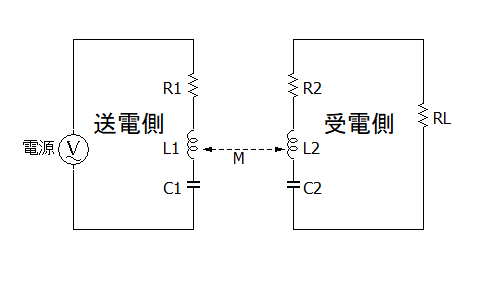
\includegraphics[]{wpt_2020128.png}
	\caption{ワイヤレス給電回路図}
	\label{fig:wpt_kairo2}
\end{figure}
図\ref{fig:wpt_kairo2}の定数と電源の値を$u$として与えると,オームの法則とキルヒホッフの法則より,
\setcounter{equation}{0}
\begin{eqnarray}
\label{eq:ohm1}
u=R_1i_1+v_1+v_2\\
\label{eq:ohm2}
(R_{L1}+R_2)i_2+v_1+v_2=0
\end{eqnarray}
 コンデンサーの電圧と電流の関係より,
\begin{eqnarray}
\label{eq:ci1}
C_1\dot{v_1}=i_1\\
\label{eq:ci2}
C_2\dot{v_2}=i_2
\end{eqnarray}
$V_{L_1}とV_{L_2}を相互インダクタンスMを含めた形にすると$
\begin{eqnarray}
\label{eq:addM1}
V_{L1}=L_1\dot{i_1}+M\dot{i_2}\\
\label{eq:addM2}
V_{L2}=M\dot{i_1}+L_2\dot{i_2}
\end{eqnarray}
式(\ref{eq:ci1})と式(\ref{eq:ci2})を変形すると,
\begin{eqnarray}
\dot{v_1}=\frac{i_1}{C_1}\\
\dot{v_2}=\frac{i_2}{C_2}
\end{eqnarray}
それぞれ式(\ref{eq:ohm1})に式(\ref{eq:addM1})を,式(\ref{eq:ohm2})に式(\ref{eq:addM2})を代入して$\dot{i}$で揃えると
\begin{eqnarray}
\label{eq:doti1}
\dot{i_1}=\frac{Mv_2-L_2v_1-R_1L_2i_1+(R_L+R_2)Mi_2+L_2u}{\Delta}\\
\label{eq:doti2}
\dot{i_2}=\frac{Mv_1-L_1v_2+MR_1i_1-(R_L+R_2)L_1i_2+Mu}{\Delta}
\end{eqnarray}
$但し\Delta は$
\begin{equation}
\Delta=L_1L_2-M^2\nonumber
\end{equation}
である.式(\ref{eq:doti1})と式(\ref{eq:doti2})を行列式でまとめると,
\begin{eqnarray}
\begin{bmatrix}
\dot{v_1}\\
\dot{v_2}\\
\dot{i_1}\\
\dot{i_2}
\end{bmatrix}
=\frac{1}{\Delta}
\begin{bmatrix}
0 & 0 & \frac{\Delta}{C_1} & 0 \\
0 & 0 & 0 & \frac{\Delta}{C_2} \\
-L_2 & M & -R_1L_2 & (R_L+R_2)M \\
M & -L_1 & R_1 & -(R_L+R_2)L_1
\end{bmatrix}
\begin{bmatrix}
v_1\\
v_2\\
i_1\\
i_2\\
\end{bmatrix}
+\frac{1}{\Delta}
\begin{bmatrix}
0\\
0\\
L_2\\
-M
\end{bmatrix}
u
\label{eq:tankei_joutai}
\end{eqnarray}
となる.この行列は以下のように$A,Bと状態変数x$として表すと,
\begin{gather}
A=\frac{1}{\Delta}
\begin{bmatrix}
0 & 0 & \frac{\Delta}{C_1} & 0 \\
0 & 0 & 0 & \frac{\Delta}{C_2} \\
-L_2 & M & -R_1L_2 & (R_L+R_2)M \\
M & -L_1 & R_1 & -(R_L+R_2)L_1
\end{bmatrix}\\
B=\frac{1}{\Delta}
\begin{bmatrix}
0\\
0\\
L_2\\
-M
\end{bmatrix}\\
x=
\begin{bmatrix}
v_1\\
v_2\\
i_1\\
i_2\\
\end{bmatrix}\\
\label{eq:zyoutai}
\dot{x}=Ax+Bu
\end{gather}
となり,式\ref{eq:zyoutai}はワイヤレス給電の状態方程式となる.
\subsection{オペアンプについて}
\begin{figure}[H]
	\centering
	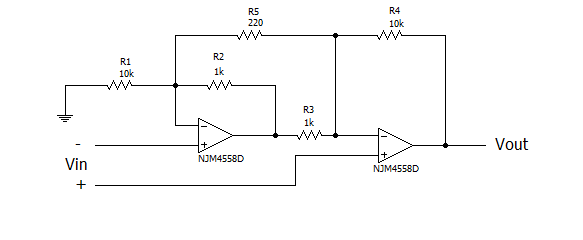
\includegraphics[]{senkou.png}
	\caption{計装用増幅回路}
	\label{fig:zouhuku}
\end{figure}
 図\ref{fig:zouhuku}のように先行研究では計装用増幅回路を組み込んだオペアンプを使用した.しかしこの回路での出力は出力前と出力後で大きなずれが生じ,乗算器でうまく乗算することができない欠点があった.また周波数を上げるほど本来上げるべき倍率である100倍にうまく出力されない欠点(周波数が高ければ高いほど出力される倍率が小さくなった)もあった.\\ そこでそこで今研究ではオペアンプを先行研究のように接続するのではなく,図(\ref{fig:hanten2})反転増幅回路を二つつなげて作った回路を使用した.また入力値と出力値とのずれを抑えるため$1000pF$程のコンデンサを入れることによりずれを防ぐようにした.
 \begin{figure}[H]
 	\centering
 	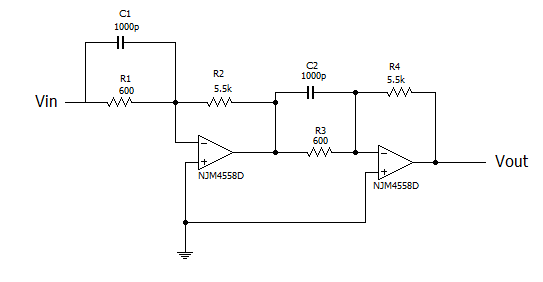
\includegraphics[]{hanten2.png}
 	\caption{反転増幅回路回路図}
 	\label{fig:hanten2}
 \end{figure}
\subsection{プログラムについて}
前章に示された通り先行研究では周波数を変更する方法で,わざわざArduinoのプログラムの一部を変更して再コンパイルさせ出力結果をシリアルモニターに表示させる方法であった.その面倒を省くためpythonを利用して周波数をarduinoに送り,arduinoの出力結果をデータに保存させるGUIを作成した.以下のプログラムはGUIで周波数をarduinoへシリアル通信で送信してarduinoに出力されたデータをシリアル通信でpython側に送る流れをするための,それぞれGUIのpythonプログラムと送電側のマイコンのarduinoプログラム,受電側のarduinoプログラムである.なお,pythonのプログラムにおいてGUIを作成にtkinterを使用した.tkinterの使用方法並びにpythonの使い方については参考文献:\cite{tkinter}を参考にした.
\lstset{
	%プログラム言語(複数の言語に対応,C,C++も可)
	backgroundcolor={\color[gray]{.90}},
	breakindent = 10pt,
	basicstyle = \ttfamily\scriptsize,
	commentstyle = {\itshape \color[cmyk]{1,0.4,1,0}},
	classoffset = 1,
	keywordstyle = {\bfseries \color[cmyk]{0,1,0,0}},
	stringstyle = {\ttfamily \color[rgb]{0,0,1}},
	frame = TBrl,
	framesep = 5pt,
	numbers = left,
	stepnumber = 1,
	numberstyle = \tiny\sffamily,
	tabsize = 4,
	captionpos = t,
	showstringspaces = false
}
	
	%直接記入の場合
	\begin{lstlisting}[caption = GUIプログラム , label = program1]
import time
import statistics
import math
import serial
import collections
import csv
import tkinter as tk
import tkinter.filedialog as tkFileDialog
import tkinter.font as tkFont
import tkinter.ttk as ttk

x=0
L=[] #dataを保存
L1=[]
L2=[]
Lmsave=[]
Lmsend=[]
Lmreceive=[]
fre=0 #測定範囲の最小値
laf=0 #1目盛りの周波数
data=0 #測定範囲の最大値
ser1=0 #送電側のシリアル通信
ser2=0 #受電側のシリアル通信
t=1
tm=0



def maindef():
global x
global L
global ser
global fre
global data
global laf
global ser1 
global ser2
global t
global tm
global L1
global L2
global Lmsave
global Lmsend
global Lmreceive

if x==0:
t=1#一応
elif x==1:
#次の周波数を入力
if float(fre) > float(laf):
x=3
else:

ser1.write('a'.encode('ascii')) # arduinoへ開始の合図を送る。
ser2.write('a'.encode('ascii'))
ser1.write(fre.encode('ascii'))
ser2.write(fre.encode('ascii'))
ser1.flush() # バッファ内の待ちデータを送りきる。
ser2.flush()
print("send:"+fre+"kHz")
L.append(fre+"kHz")
x=2
t=1
elif x==2:
#データ受け取りスイープ
line1 = ser1.readline().decode('ascii').rstrip()
line2 = ser2.readline().decode('ascii').rstrip()
L1.append(line1)
L2.append(line2)
print(fre+" "+line1+" "+line2+" ")
L.append(fre+" "+line1+" "+line2+" ")
if t>=int(tm):
math1=collections.Counter(L1).most_common()[0][0]
math2=collections.Counter(L2).most_common()[0][0]
Lmsave.append(fre+" "+math1+" "+math2)
Lmsend.append(fre+" "+math1)
Lmreceive.append(fre+" "+math2)
if float(fre)+float(data)*0.001 > float(laf) and float(laf) > float(fre):
fre=laf
else:
fre=str(round(float(fre) + float(data)*0.001,3))
x=1
L1=[]
L2=[]
else:
t=t+1

elif x==3:
#データを送らない、後始末
stop_data()
x=0
elif x==4:
#データ受け取り通常
line1 = ser1.readline().decode('ascii').rstrip()
line2 = ser2.readline().decode('ascii').rstrip()
print(fre+" "+line1+" "+line2+" ")
L.append(fre+" "+line1+" "+line2+" ")

root.after(10,maindef)

class Ser:
def __init__(self):
self.ser=None

def start_connect(self):
global ser1
global ser2
comport1='COM4' # arduino ideで調べてから。送電側
comport2='COM3' #受電側必ずcomportは送電側受電側異なるものを使用
tushinsokudo=57600 # arduinoのプログラムと一致させる。
timeout=5# エラーになったときのために。とりあえず5秒で戻ってくる。
ser1=self.ser
ser2=self.ser
ser1 = serial.Serial(comport1,tushinsokudo,timeout=timeout)
ser2 = serial.Serial(comport2,tushinsokudo,timeout=timeout)
time.sleep(2) # 1にするとダメ!短いほうがよい。各自試す。

def send_com(self):
global x
global data
global fre
global laf
global ser1
global ser2
global L
global tm
global L1
global L2
global Lmsave
global Lmsend
global Lmreceive
# v,u,sの文字列は、
#ぞれぞれv.get(),u.get(),s.get()で取り出す。
#下部send_entry内のTextvariableでデータ入力
data=v.get()
fre=u.get() 
laf=s.get()
tm=v1.get() 
if data.isdecimal()==True and fre.isdecimal()==True and laf.isdecimal()==True and tm.isdecimal()==True:
ser1.write('a'.encode('ascii')) # arduinoへ開始の合図を送る。
ser2.write('a'.encode('ascii'))
ser1.write(fre.encode('ascii'))
ser2.write(fre.encode('ascii'))#送電側と受電側の送るデータの量を合わせるため,
#あえて周波数を送る.送らなかった場合,送電側と受電側の出力にずれが生じるから.
ser1.flush() # バッファ内の待ちデータを送りきる。
ser2.flush()
print("send incease_fre:"+data+" first_fre:"+fre+" last_fre:"+laf)
print("frequency transmission_ep receiving_ep")
L.append("increase_frequency:"+data+" first_frequency:"+fre+" last_frequency:"+laf)
L.append("frequency transmission_ep receiving_ep")
print("send:"+fre+"kHz")
L.append(fre+"kHz")
L1=[]
L2=[]
Lmsave=[]
Lmsend=[]
Lmreceive=[]


if int(data)==0:
x=4
else:
x=2
t=1
else:
print("error")
v.set("")
u.set("")
s.set("")
v1.set("")
def stop_com(self):
global x
x=3


def connect(self):
self.start_connect()
send_button.configure(state=tk.NORMAL)
stop_button.configure(state=tk.NORMAL)
send_entry.configure(state=tk.NORMAL)
defalt_entry.configure(state=tk.NORMAL)
saveas_button.configure(state=tk.NORMAL)
max_entry.configure(state=tk.NORMAL)
time_entry.configure(state=tk.NORMAL)
connect_button.configure(state=tk.DISABLED)
saveas_combo.configure(state=tk.NORMAL)

def saveas():
global L
global data
global Lmreceive
global Lmsave
global Lmsend
secomb=vc.get()
if secomb=='all':
save(L)
else:
if data=='0':
print("error!!")
else:
if secomb=='sweep:fre-send-receive':
save(Lmsave)
elif secomb=='sweep:fre-send':
save(Lmsend)
elif secomb=='sweep:fre-receive':
save(Lmreceive)

def save(a):
filename=tkFileDialog.asksaveasfilename(defaultextension=".csv",filetypes=[("csv","*.csv*")])
with open(filename,'w') as fout:
fout.write("\n".join(a))


#周波数をclock_genelaterに送る
#ストップするときの関数
def stop_data():
global ser1
global ser2
global fre
ser1.write('b'.encode('ascii')) # arduinoへ終了の合図を送る。
ser2.write('b'.encode('ascii'))
ser1.flush() # バッファ内の待ちデータを送りきる。
ser2.flush()
ser1
print("--stop--")
L.append("stop")
fre='0'
time.sleep(1)

root=tk.Tk()
font=tkFont.Font(size=24)
ser=Ser() 
v=tk.StringVar() # tk.TK()の後に書く。
u=tk.StringVar()
s=tk.StringVar()
v1=tk.StringVar()
vc=tk.StringVar()

#ボタン入力
connect_button=tk.Button(root,text='connect',font=font,height=2,padx=20,command=ser.connect)
connect_button.grid(row=0,column=0)
send_button=tk.Button(root,text='send',font=font,height=2,padx=20,command=ser.send_com)
send_button.grid(row=0,column=1)
send_button.configure(state=tk.DISABLED)
stop_button=tk.Button(root,text='stop',font=font,height=2,padx=20,command=ser.stop_com)
stop_button.grid(row=0,column=2)
stop_button.configure(state=tk.DISABLED)
#entry
send_entry=tk.Entry(root,font=font,textvariable=v)
send_entry.grid(row=1,column=1,columnspan=2)
send_entry.configure(state=tk.DISABLED)
defalt_entry=tk.Entry(root,font=font,textvariable=u)
defalt_entry.grid(row=2,column=1,columnspan=2)
defalt_entry.configure(state=tk.DISABLED)
max_entry=tk.Entry(root,font=font,textvariable=s)
max_entry.grid(row=3,column=1,columnspan=2)
max_entry.configure(state=tk.DISABLED)
time_entry=tk.Entry(root,font=font,textvariable=v1)
time_entry.grid(row=4,column=1,columnspan=2)
time_entry.configure(state=tk.DISABLED)

#label
label1=tk.Label(root,font=font,text='increase_frequency')
label1.grid(row=1,column=0)
label1_Hz=tk.Label(root,font=font,text='Hz')
label1_Hz.grid(row=1,column=3)
label2=tk.Label(root,font=font,text='first_frequency')
label2.grid(row=2,column=0)
label2_Hz=tk.Label(root,font=font,text='kHz')
label2_Hz.grid(row=2,column=3)
label3=tk.Label(root,font=font,text='last_frequency')
label3.grid(row=3,column=0)
label3_Hz=tk.Label(root,font=font,text='kHz')
label3_Hz.grid(row=3,column=3)
label4_time=tk.Label(root,font=font,text='Measurement_Time')
label4_second=tk.Label(root,font=font,text='ds')
label4_time.grid(row=4,column=0)
label4_second.grid(row=4,column=3)

#セーブボタン
saveas_button=tk.Button(root,text='save',font=font,height=2,padx=20,command=saveas)
saveas_button.grid(row=0,column=3)
saveas_button.configure(state=tk.DISABLED)

#COMBOBOX
Comb=['all','sweep:fre-send-receive','sweep:fre-send','sweep:fre-receive']
saveas_combo=ttk.Combobox(root,values=Comb,textvariable=vc)
vc.set(Comb[0])
saveas_combo.grid(row=0,column=4)
saveas_combo.configure(state=tk.DISABLED)

root.after(100,maindef)
root.mainloop()   
	\end{lstlisting}
	\begin{lstlisting}[caption=送電側arduino, label=program2]

#include <si5351.h>
#include <Wire.h>
#include<MsTimer2.h>
Si5351 si5351;

unsigned long long freq = 5000000ULL;           
/*出力周波数50kHz(これをいじって周波数を変える)freq×0.01=周波数Hz*/
unsigned long long pll_freq = 70500000000ULL;   /*PLL周波数(いじるな)*/

String data;
float data0 = 0;
float f = 0;

void setup() {

Serial.begin(57600);
MsTimer2::set(100, flash);

bool i2c_found;                                         
/*I2C通信ができるかどうかブール値を入れる変数*/
i2c_found = si5351.init(SI5351_CRYSTAL_LOAD_8PF, 0, 0); 
 /*I2C通信を確認(ライブラリreadme参照)*/
if (!i2c_found) {
Serial.println("Error:I2C");
}

si5351.init(SI5351_CRYSTAL_LOAD_8PF, 0, 0);            
 /*振動子負荷容量(使うモジュールが8pFなのでこれ)*/
si5351.set_freq_manual(freq, pll_freq, SI5351_CLK0);   
 /*出力周波数,PLL周波数,設定先出力ピン設定*/
si5351.set_phase(SI5351_CLK0, 0);                      
 /*位相(今回特に意味はない)*/
si5351.pll_reset(SI5351_PLLA);                         
 /*PLLをリセット(使う前に一回リセット)*/
si5351.update_status();                                
 /*si5351のステータスを読む(今回特に使っていない)*/

while (Serial.available() == 0);
}




void flash(void) {
int i = analogRead(0);
f = i * 5.0 / 1023.0;
Serial.println(f,4);
//有効数字を4桁にする.
//シリアルモニターは初期設定では小数第二位までしか読み取れないから.
}

void loop() {
char aizu = Serial.read();
if (aizu == 'a') {
MsTimer2::stop(); //新しいduty比に変更されるまでflash関数を止める
aizu = 'c';
receive_duty_data();
MsTimer2::start();
}

else if (aizu == 'b') {
MsTimer2::stop();
si5351.set_freq(400000, SI5351_CLK0);  
  /*信号を止める*/            /*!!!!!set_freq(0)!!!これでは止まらない!!!!!*/
}

else if (aizu == 'c') {
//pass
}
}

void receive_duty_data() {
data = Serial.readString();
data0 = data.toFloat();
unsigned long long freq = data0 * 100000; 
/*1=0.01Hzなので末尾に00をつける.入力単位をキロにしたいので末尾に10^3をつける.*/
si5351.set_freq(freq, SI5351_CLK0);       /*周波数セット*/
si5351.pll_reset(SI5351_PLLA);            /*念のためPLLをリセット*/
si5351.update_status();
}
	
	\end{lstlisting}
	\begin{lstlisting}[caption=受電側arduino, label=program3]
#include<MsTimer2.h>
float f = 0;
String data;
float data0 = 0;
void setup() {
Serial.begin(57600);
MsTimer2::set(100,flash);
while(Serial.available() == 0);
}
void flash(void){
int i = analogRead(0);
f = i * 5.0 / 1023.0;
Serial.println(f,4);
//有効数字を4桁にする.
//シリアルモニターは初期設定では小数第二位までしか読み取れないから.
}
void loop() {
char aizu = Serial.read();
if(aizu == 'a'){
MsTimer2::stop();
aizu = 'c';
receive_duty_data();
MsTimer2::start();
}
else if(aizu == 'b'){
MsTimer2::stop();
aizu='c';
}

}
void receive_duty_data() {

data = Serial.readString();
data0 = data.toFloat();
}
	\end{lstlisting}

\end{document}

